%% Project Documentation
%% Based on elsarticle template (Elsevier Ltd, 2009)

\documentclass[final,3p,times,twocolumn]{elsarticle}

\usepackage{amssymb}
\usepackage{lineno}
\usepackage{graphicx}
\usepackage[hidelinks]{hyperref}
\usepackage{tabularx}
\usepackage{multirow}
\usepackage{listings}
\usepackage{xcolor}
\usepackage{tikz}
\usetikzlibrary{positioning}

\journal{KIV/VI - Information Visualization}

\begin{document}

\begin{frontmatter}

\title{Interactive Visualization Platform for Informatics Education Statistics Across European Universities}

\author{Bc. Břetislav Milota, Bc. Martin Schön}

\address{Department of Computer Science and Engineering, Faculty of Applied Sciences, University of West Bohemia, Plze\v{n}, Czech Republic}

\begin{abstract}
This paper presents a semester project on developing an interactive web-based application for exploring informatics education data across European institutions. The platform integrates geographic mapping, choropleth visualizations, and statistical charts to enable analysis of student enrollment, graduation rates, and female representation at both country and institutional levels. 
Data from Informatics Europe (IE) member institutions, the European Tertiary Education Register (ETER), and manually curated sources are processed by a Python pipeline into static JSON files consumed by a Vue~3 single-page application. The system allows users to search and filter over 200 institutions, compare any two countries or institutions side by side, and examine trends across Bachelor's, Master's, and doctoral programmes.
\end{abstract}

\begin{keyword}
information visualization \sep educational statistics \sep Informatics Europe \sep choropleth maps \sep Vue.js \sep interactive maps
\end{keyword}

\end{frontmatter}

%\linenumbers

% -------------------------------------------------------
\section{Introduction}
% -------------------------------------------------------

Understanding the state of informatics education across Europe is critical for academics, policy makers, and institutions that wish to benchmark their performance and identify structural trends. Informatics Europe (IE) is the professional association of computer science and informatics research and education institutions in Europe, and it maintains a network of member universities along with time-series data on student enrollment, degrees awarded, and female representation at Bachelor's, Master's, and doctoral levels.

Despite the richness of this dataset, it is currently stored in Excel spreadsheets and accessed through manual queries, making it difficult to identify geographic patterns, compare institutions across countries, or observe multi-year trends without significant manual effort. The same challenge applies to the European Tertiary Education Register (ETER), a comprehensive registry of European higher-education institutions that provides enrollment and graduation statistics across all disciplines but requires specialist tooling to navigate.

This work addresses these limitations by providing a unified, browser-based interface that transforms raw spreadsheet data into interactive visualizations. The application serves researchers, university administrators, and IE staff who need accessible, visual insight into the state of informatics education across Europe.

The contributions of this work are:
\begin{itemize}
    \item A Vue~3 single-page application integrating geographic and statistical visualizations in a single interface.
    \item A modular Python data pipeline that aggregates and geocodes data from multiple heterogeneous sources.
    \item A side-by-side comparison view enabling simultaneous analysis of any two countries or institutions.
    \item A choropleth layer offering nine configurable dataset/metric combinations with per-capita normalization.
\end{itemize}

% -------------------------------------------------------
\section{Related Work}
\label{sec:relatedwork}
% -------------------------------------------------------

This section reviews work related to three aspects of this project: existing platforms for exploring higher-education data in Europe, research on the gender gap in informatics education that motivates the gender-focused visualizations, and established techniques in geospatial and statistical visualization that informed the design choices made in this work.

\subsection{Existing Higher-Education Data Portals}

The Informatics Europe Higher Education Data Portal~\cite{IEPortal2023} is the system most closely related to this work. Launched in 2019 in collaboration with the Software Institute at Università della Svizzera italiana, it exposes the same Members-DATA workbook through a web interface offering tabular views and basic charts. However id does not provide geographic map views, choropleth overlays, or institution-level geocoding, limiting a user's ability to identify spatial patterns and regional disparities. This work can be understood as a geospatial and statistical complement to this portal.

The European Tertiary Education Register (ETER)~\cite{Lepori2023} is a pan-European reference dataset covering approximately 3,500 higher-education institutions across 41 countries, collected in compliance with OECD-UNESCO-EUROSTAT standards by national statistical authorities. The ETER web interface supports tabular downloads and basic filtering but provides no integrated visualization layer. This work integrates ETER enrollment and graduation records alongside IE member statistics, presenting both through a common interface.

The European Higher Education Sector Observatory (EHESO) is a newer platform built on top of ETER that introduces dashboards and scorecards for evidence-based policy making. While it offers more visualization than the raw ETER portal, its scope is broad across all disciplines and institutions, and it does not specialize in the informatics domain or in the IE member network.

\subsection{Gender Balance in Informatics Education}

The gender gap in informatics higher education in Europe is a well-documented problem. The EUGAIN COST Action~\cite{EUGAIN2024} coordinates research and best-practice exchange across more than 30 countries. A recent EUGAIN-funded study~\cite{DAngelo2024} specifically analyzed female participation trends in European informatics degrees using the IE data portal as its primary source, finding that in the majority of European countries more than 80\% of informatics bachelor students are male, and that this ratio has changed little over the past decade. By using a choropleth layer and per-institution modal charts make these trends immediately visible without requiring manual data extraction.

\subsection{Geospatial and Statistical Visualization Techniques}

Choropleth maps are an established method for communicating spatial distributions of statistical indicators. A systematic evaluation of choropleth augmentation strategies~\cite{Choropleth2020} found that juxtaposed linked maps and synchronized interactions are among the most effective approaches for comparative multi-variable analysis. This work adopts a single configurable choropleth layer supplemented by a detail modal, avoiding the visual clutter of overlapping encodings while supporting comparison through a dedicated side-by-side view.

Leaflet~\cite{Leaflet} has become the de facto open-source JavaScript library for browser-based interactive mapping and is used in institutional and governmental portals worldwide. Its lightweight footprint and plugin ecosystem, including the MarkerCluster extension employed by this work, make it well-suited to static-serving deployments. Statistical charting is handled by Chart.js~\cite{ChartJS}, a widely adopted canvas-based library for responsive bar, line, and doughnut charts in web applications.

% -------------------------------------------------------
\section{Methods}
\label{sec:methods}
% -------------------------------------------------------

This section describes how the application was designed and implemented. It covers the overall system architecture, the offline Python data pipeline responsible for collecting and transforming raw data into static JSON files, the frontend Vue components that render those files as interactive maps and charts, the data sources integrated by the system, and the deployment setup.

\subsection{System Architecture}

This work follows a strict separation between an offline data pipeline and a static frontend application. No server-side computation is performed at runtime; all processing occurs during an offline data-generation phase that produces JSON files deployed alongside the frontend bundle. This architecture simplifies deployment (a single nginx container) and allows the frontend to operate without any backend infrastructure.

Figure~\ref{fig:architecture} outlines the data flow from raw sources to the user interface.

\begin{figure*}[t]
\centering
\resizebox{\textwidth}{!}{%
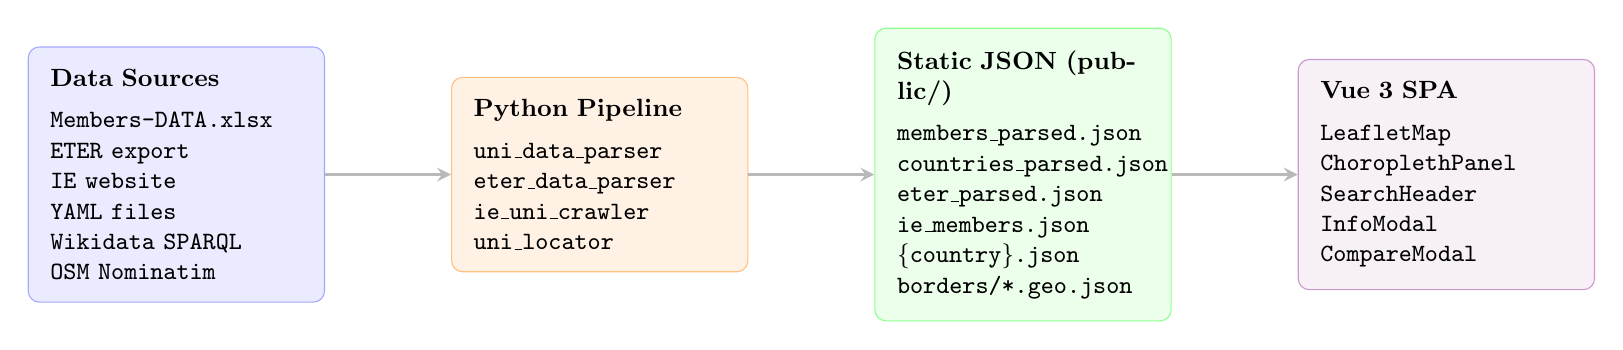
\begin{tikzpicture}[
  font=\small,
  >=stealth,
  box/.style={
    draw, rounded corners=4pt,
    inner sep=8pt,
    align=left,
    text width=3.2cm
  }
]

\node[box, fill=blue!8, draw=blue!35] (src) {
  {\bfseries Data Sources}\\[4pt]
  \texttt{Members-DATA.xlsx}\\
  \texttt{ETER export}\\
  \texttt{IE website}\\
  \texttt{YAML files}\\
  \texttt{Wikidata SPARQL}\\
  \texttt{OSM Nominatim}
};

\node[box, fill=orange!10, draw=orange!50, right=1.6cm of src] (pipe) {
  {\bfseries Python Pipeline}\\[4pt]
  \texttt{uni\_data\_parser}\\
  \texttt{eter\_data\_parser}\\
  \texttt{ie\_uni\_crawler}\\
  \texttt{uni\_locator}
};

\node[box, fill=green!8, draw=green!45, right=1.6cm of pipe] (json) {
  {\bfseries Static JSON (public/)}\\[4pt]
  \texttt{members\_parsed.json}\\
  \texttt{countries\_parsed.json}\\
  \texttt{eter\_parsed.json}\\
  \texttt{ie\_members.json}\\
  \texttt{\{country\}.json}\\
  \texttt{borders/*.geo.json}
};

\node[box, fill=violet!6, draw=violet!40, right=1.6cm of json] (vue) {
  {\bfseries Vue~3 SPA}\\[4pt]
  \texttt{LeafletMap}\\
  \texttt{ChoroplethPanel}\\
  \texttt{SearchHeader}\\
  \texttt{InfoModal}\\
  \texttt{CompareModal}
};

\draw[->, very thick, gray!55] (src.east)  -- (pipe.west);
\draw[->, very thick, gray!55] (pipe.east) -- (json.west);
\draw[->, very thick, gray!55] (json.east) -- (vue.west);

\end{tikzpicture}%
}
\caption{Diagram of data flow. Offline Python scripts transform raw data from Excel, YAML, and web sources into static JSON files. The Vue~3 SPA fetches these files at runtime and renders them as interactive maps and charts.}
\label{fig:architecture}
\end{figure*}

\subsection{Data Pipeline}

The pipeline consists of four independent Python scripts, each responsible for one data domain:

\textbf{IE Member Crawler} (\texttt{ie\_uni\_crawler/}): Scrapes the Informatics Europe website using \texttt{requests} and \texttt{lxml} XPath selectors to extract the current list of member institutions. Each institution is then geocoded via the OpenStreetMap Nominatim API to obtain coordinates. The output is \texttt{ie\_members.json}.

\textbf{University Data Parser} (\texttt{uni\_data\_parser/}): Reads the \texttt{Members-DATA} Excel workbook using \texttt{pandas} and \texttt{openpyxl}. It extracts per-institution BSc, MSc, and PhD statistics (total enrolled, first-year cohort, degrees awarded, female counts) across all available years. Country-level aggregates are computed and population data is fetched from the Wikidata SPARQL endpoint to enable per-capita metrics. Outputs are \texttt{members\_parsed.json} and \texttt{countries\_parsed.json}.

\textbf{ETER Data Parser} (\texttt{eter\_data\_parser/}): Reads the ETER export files\footnote{Data available at: \url{https://eter-project.com/data/data-for-download-and-visualisations/database/}} and reconciles institution names with the IE member list using fuzzy string matching (\texttt{thefuzz} library) to link ETER enrollment and graduation records to known IE institutions. Output is \texttt{eter\_parsed.json}.

Not all ETER columns are retained — only fields relevant to the application are extracted. Table~\ref{tab:eter_fields} in the Attachments lists the selected fields grouped by category.

\textbf{University Locator} (\texttt{uni\_locator/}): Processes manually curated YAML files for countries (Czech Republic, Germany, Norway, Portugal, Latvia) are used to identify and geocode individual departments within universities. Outputs are per-country GeoJSON files in \texttt{public/unis/}.

\textbf{Country Border Fetcher}: Country boundary polygons used by the choropleth and leaflet layers are sourced from the GeoJSON Maps service\footnote{\url{https://geojson-maps.kyd.au/}} at the highest available resolution (10m precision). Each country's border is downloaded as a separate GeoJSON file and stored in \texttt{public/borders/}, keeping the per-country files independent so that only the borders of currently visible countries need to be loaded by the frontend at runtime.

\subsection{Frontend Application}

The frontend is built with Vue~3 and TypeScript, bundled with Vite, and served in production by nginx on Alpine Linux via a two-stage Docker build.

\textbf{Interactive Map} (\texttt{LeafletMap.vue}): The central component renders a Leaflet~1.9 map with two toggleable marker layers: standard institutions (blue), IE member institutions (green). When institution is selected marker will be red. Markers are clustered using the Leaflet.markercluster plugin to handle dense regions. Clicking a marker opens the detail modal for that institution. A \textit{fly-to} animation is triggered when the user selects an item from the search results.

\textbf{Choropleth Panel} (\texttt{ChoroplethPanel.vue} + \texttt{useChoropleth.ts}): Country boundaries are loaded as GeoJSON and colored according to a selected dataset (BSc/MSc/PhD $\times$ enrolled/first-year/degrees awarded) and metric (total count, female count, female share, or count per~$10^6$ population). A diverging color scale maps values to a gradient from light to saturated hue. The year selector auto-detects the most data-complete year for the chosen dataset.

\textbf{Search and Filtering} (\texttt{SearchHeader.vue}): A real-time text search queries a flat list of all universities and departments. Results are filtered by country (dropdown) and IE-membership status (toggle). IE members are indicated with a star icon in the results list.

\textbf{Detail and Comparison Modals} (\texttt{InfoModal.vue}, \texttt{CompareModal.vue}): Opening a country or institution triggers a modal that dynamically loads parsed data and renders statistical charts using Chart.js. Visual encodings are chosen to suit each variable:
\begin{itemize}
    \item \textbf{Stacked bar charts} decompose total enrollment into constituent cohorts. For BSc programs, bars distinguish incoming first-year students from returning cohorts to illustrate retention; for European-context views, bars represent aggregate enrollment across BSc, MSc, and PhD programs per country.
    \item \textbf{Line charts} track time-series data profile variables over time, including total degrees awarded per year and the percentage of female students across degree levels.
    \item \textbf{Doughnut charts} visualize each country's proportional share of the total European student population for a selected academic year.
    \item \textbf{Normalized density} is computed by dividing raw student totals by Wikidata current population figures, yielding a students-per-million metric that reveals institutional coverage independently of country size.
\end{itemize}
The comparison mode renders two independent chart sets side by side for any selected pair of countries or institutions. Color hue differentiates degree levels (e.g., blue for BSc, orange for MSc) while line style (solid vs.\ dashed) distinguishes the two compared entities.

\subsection{Data Sources}

Table~\ref{tab:sources} in the Attachments summarises the data sources integrated by this application.

\subsection{Deployment}

Production deployment uses Docker Compose. The \texttt{docker-compose.yml} defines a single service that builds the Vue application inside a Node~22 container and copies the compiled artefact to an nginx:alpine image, which serves it on port~80 mapped to host port~8080.

% -------------------------------------------------------
\section{Results}
\label{sec:results}
% -------------------------------------------------------

The deployed application visualizes informatics education data across Europe. The following subsections describe the key visualizations produced by the system. All figures are collected in the Attachments. National-level charts use France as a reference country; institution-level charts use the Instituto Polit\'{e}cnico de Leiria (Portugal).

\subsection{Interactive Map and Choropleth}

The primary entry point is a full-screen interactive map (Figure~\ref{fig:europe_map}) built with Leaflet. University markers are clustered automatically at lower zoom levels, giving an immediate overview of institutional density across the continent; clusters expand on zoom or click to reveal individual institutions. Figure~\ref{fig:cz_map} shows the same view zoomed into the Czech Republic, where department-level markers become individually visible.

The choropleth panel overlays country boundaries with a color scale driven by the selected dataset and metric. Figures~\ref{fig:choropleth_2010} and~\ref{fig:choropleth_2023} compare the absolute female student count at BSc level between the 2010/11 and 2023/24 academic years. The shift in color intensity across most countries reflects growth in absolute female enrollment over the 13-year period, though the relative share has remained largely stagnant as overall enrollment grew proportionally.

\subsection{National Profile and Output Trends}

The country detail modal exposes a country's educational profile across all available years. Figure~\ref{fig:enrollment} shows the \textit{Enrollment Trends} chart, a stacked bar chart that separates incoming first-year students from returning cohorts for BSc programs, making retention patterns visible. MSc and PhD enrollments are rendered as standard single-bar charts.

Figure~\ref{fig:degrees} tracks \textit{Degrees Awarded} over time via a line chart, providing a view of a country's time-series data academic output. 

\subsection{Country Female Representation}

Figure~\ref{fig:female_rep} visualizes the \textit{Trend in Female Representation}, plotting the percentage of female students at BSc and MSc level over time and explicitly exposing persistent disparities between degree pipelines. The chart uses separate lines for BSc and MSc to make it immediately apparent whether the gender ratio differs between programme levels within the same country — a pattern that is not visible from enrollment totals alone. This visualization directly complements the choropleth layer: while the map shows which countries have higher female counts in a given year, this chart reveals whether those counts represent a genuine long-term trend or a short-term fluctuation.

\subsection{European Context and Institutional Density}

The European Context tab presents three comparative visualizations for a selected academic year. Figure~\ref{fig:doughnut} shows the \textit{European Student Distribution} as a doughnut chart, illustrating each country's share of the total European informatics student population.

Figure~\ref{fig:absolute} presents the \textit{Absolute Scale} view — a stacked bar chart of raw enrollment totals per country. Highly populous nations such as Germany, the UK, Turkey, and Italy dominate this view. Figure~\ref{fig:density} shows the \textit{National Density} view, where totals are normalized per one million inhabitants. This transformation reveals that smaller nations --- Sweden, Finland, Greece, and Estonia --- have significantly higher concentrations of informatics students relative to their population, a pattern completely obscured by the absolute-scale view.

\subsection{Institutional Sizing and Output}

At the institutional level, the detail modal provides sizing metrics from two sources. Figure~\ref{fig:inst_ie} shows the \textit{Student Enrollment} chart from the Members-DATA source, using a grouped bar chart to compare total enrollment against female enrollment across degree levels for a single academic year. This view is available only for the small subset of institutions that report to Informatics Europe.

Figure~\ref{fig:inst_eter} tracks \textit{Enrollment Over Time} from the ETER registry using side-by-side bars to contrast BSc and MSc enrollment fluctuations across years. Figure~\ref{fig:inst_grad} extends this with a \textit{Graduates Over Time} line chart, revealing institutional output trajectories over a multi-year period.

\subsection{Side-by-Side Benchmarking}

When user selects some country or institution, the detail modal includes a \textit{Compare} button that opens a side-by-side view. There users can select any other country or institution to compare against the base entity.

The comparison view allows users to select any two countries or institutions and view their profile variables in parallel. Figure~\ref{fig:cmp_enroll} shows \textit{Total Enrollment Comparison} between two countries using grouped, color-coded bar charts. Figure~\ref{fig:cmp_degrees} extends this to academic output via comparative line charts. Figure~\ref{fig:cmp_female} demonstrates \textit{Female Representation Comparison}, handling four simultaneous data series (BSc and MSc for two countries) using color hue to differentiate degree levels and line style (solid vs.\ dashed) to distinguish the two compared entities.

% -------------------------------------------------------
\section{Discussion}
\label{sec:discussion}
% -------------------------------------------------------

This section reflects on the outcomes of this work in a broader context. It first compares the application against the related systems identified in Section~\ref{sec:relatedwork}, highlighting where this work adds value and where it deliberately stays out of scope. It then examines how the gender-gap findings from the literature are made visible through the platform's visualizations. Finally, it addresses the current limitations of the system — data coverage gaps, pipeline constraints, and architectural trade-offs — that future work should consider.

\subsection{Comparison with Related Systems}

This work differs from the existing IE Higher Education Data Portal~\cite{IEPortal2023} primarily in its geographic dimension. Whereas the portal presents data through country-level tables and static charts, this application places every institution on an interactive map and links it to its statistical profile. The choropleth layer makes cross-country comparisons immediate, which is not possible in the tabular portal interface. At the same time, this work does not aim to replace the portal: it does not expose the full range of salary, staffing, or funding indicators available there, focusing instead on the enrollment, graduation, and gender metrics that benefit most from spatial and temporal visualization.

Compared to EHESO~\cite{Lepori2023}, this work is narrower in disciplinary scope (informatics only) but deeper in the IE-specific layer: geocoded departments, IE membership status, and the Members-DATA statistics are not surfaced in EHESO. The two systems are therefore complementary rather than competing.

\subsection{Gender Gap Visibility}

The platform makes the findings of~\cite{DAngelo2024} directly accessible to non-specialist users. Loading the choropleth with the female-share metric at bachelor level immediately reveals that the majority of European countries fall below the 25\% threshold. The year-by-year animation (proposed in Section~\ref{sec:futurework}) would further expose the slow pace of change over the 14-year dataset window.

\subsection{Limitations}

\textbf{Data latency and manual pipeline.} The Python scripts must be run manually whenever source data changes. The Members-DATA workbook is updated annually, and ETER data may lag by two or more years. The platform therefore always presents a snapshot rather than a live picture of the state of informatics education.

\textbf{Coverage gaps.} The Members-DATA workbook covers only IE member institutions. Non-member universities, which may include large national players, are absent from the member-level statistics. ETER broadens the institutional scope but is limited to the countries and years for which national statistical authorities have supplied data.

\textbf{Name-matching reliability.} Fuzzy string matching used to link ETER records to IE members introduces a risk of false positives when institutions have similar names. No automated verification step currently validates matched pairs.

\textbf{Manual YAML curation.} Department-level data for the Czech Republic, Germany, Norway, Portugal, and Latvia depends on hand-maintained YAML files. Keeping these current requires editorial effort that scales poorly as the number of covered countries grows.

\textbf{Static deployment.} The single-page application architecture simplifies hosting but prevents server-side filtering, pagination, or user-specific state that would be needed to support a significantly larger dataset or more complex query patterns.

% -------------------------------------------------------
\section{Future Work}
\label{sec:futurework}
% -------------------------------------------------------

Several directions could extend the current platform:

\textbf{Automated data refresh}: The pipeline currently requires manual invocation whenever source data changes. Scheduling the Python scripts via CI/CD and publishing updated JSON artefacts automatically would keep the platform current without human intervention.

\textbf{Broader geographic coverage}: YAML-based manual data entry is required for countries not fully covered by the Members-DATA workbook. Integrating additional national data registries or expanding IE data coverage would reduce this manual burden.

\textbf{Institution-type breakdown}: The ETER dataset distinguishes Research Universities from Universities of Applied Sciences, but this dimension is not yet surfaced as a filter in the UI. Exposing it would allow more targeted comparisons.

\textbf{Time-series animation}: A playback control that animates the choropleth layer year by year would make temporal trends immediately apparent without manual year-by-year navigation.

\textbf{Mobile optimization}: The current layout is designed for desktop browsers. Responsive breakpoints and touch-friendly controls for the map and modals would improve usability on smaller screens.

\textbf{Export functionality}: Allowing users to export filtered datasets as CSV or the current chart view as PNG or PDF would improve the platform's utility for researchers preparing reports.

% -------------------------------------------------------
\section*{Acknowledgement}
% -------------------------------------------------------

We would like to thank Informatics Europe for maintaining and sharing the Members-DATA workbook, the ETER consortium for providing open access to the European Tertiary Education Register, and the OpenStreetMap community for the Nominatim geocoding service.

%% References
\bibliographystyle{elsarticle-num-names}
\bibliography{BibTexReferences}

\newpage
% -------------------------------------------------------
\section*{Attachments}
% -------------------------------------------------------

The following pages contain all tables and figures referenced throughout the text, presented in the order they appear in the paper. Tables are listed first, followed by all visualizations.

\begin{table*}[htbp]
\caption{Data sources and their roles in this work.}
\label{tab:sources}
\begin{tabularx}{\textwidth}{lX}
\hline
\textbf{Source} & \textbf{Role} \\
\hline
Informatics Europe website & IE member list \\
Members-DATA Excel & Per-institution statistics (BSc, MSc, PhD enrollment, degrees awarded, female counts) \\
ETER export & EU-wide enrollment and graduation data across all higher-education institutions \\
YAML files (\texttt{data/}) & Manually curated department-level data for CZ, DE, NO, PT, LV \\
Wikidata SPARQL & Country population figures for per-capita normalization \\
OSM Nominatim API & University and department geographic coordinates \\
\hline
\end{tabularx}
\end{table*}

\begin{table*}[htbp]
\caption{ETER fields extracted by the data parser.}
\label{tab:eter_fields}
\begin{tabularx}{\textwidth}{llX}
\hline
\textbf{Category} & \textbf{Field} & \textbf{Purpose} \\
\hline
\multirow{6}{*}{Identity} & ETER ID & Unique stable identifier for each institution \\
 & Institution Name & Official name in the national language \\
 & English Institution Name & Standardised English name for display \\
 & Country Code & ISO country code used for map and filter matching \\
 & Reference Year & Academic year, used to populate the year selector \\
 & Institution Category (standardised) & Type: Research University, University of Applied Sciences, etc. \\
\hline
\multirow{3}{*}{Geography} & City Name & City of the main campus \\
 & Latitude & Geographic coordinate for Leaflet marker placement \\
 & Longitude & Geographic coordinate for Leaflet marker placement \\
\hline
\multirow{4}{*}{BSc Graduates (ISCED~6)} & Graduates in ICT & Total ICT graduates at bachelor level \\
 & Graduates --- men & Male ICT graduates at bachelor level \\
 & Graduates --- women & Female ICT graduates at bachelor level \\
 & Total graduates & All-discipline total (used to compute ICT share) \\
\hline
\multirow{4}{*}{MSc Graduates (ISCED~7)} & Graduates in ICT & Total ICT graduates at master level \\
 & Graduates --- men & Male ICT graduates at master level \\
 & Graduates --- women & Female ICT graduates at master level \\
 & Total graduates & All-discipline total (used to compute ICT share) \\
\hline
\end{tabularx}
\end{table*}

\begin{figure*}[htbp]
    \centering
    \includegraphics[width=0.92\linewidth]{images/europe_map.png}
    \caption{Interactive map of Europe showing all universities and departments as clustered markers. Cluster size reflects the number of institutions in the area; clusters expand on zoom or click to reveal individual markers. Blue markers represent general institutions, green markers indicate IE members. In this view the IE member institutions and other institutions are clustered together.}
    \label{fig:europe_map}
\end{figure*}

\begin{figure*}[htbp]
    \centering
    \includegraphics[width=0.92\linewidth]{images/cs_map_focus.png}
    \caption{Interactive map zoomed into the Czech Republic. At this zoom level individual department-level markers become visible, revealing the geographic distribution of informatics departments within the country.}
    \label{fig:cz_map}
\end{figure*}

\begin{figure*}[htbp]
    \centering
    \includegraphics[width=0.92\linewidth]{images/color_map_female_10-11.png}
    \caption{Choropleth map showing the absolute number of female BSc informatics students per country in the 2010/11 academic year. The greener the color, the higher the count. Countries with no available data are shown in grey.}
    \label{fig:choropleth_2010}
\end{figure*}

\begin{figure*}[htbp]
    \centering
    \includegraphics[width=0.92\linewidth]{images/color_map_female_23-24.png}
    \caption{Choropleth map showing the absolute number of female BSc informatics students per country in the 2023/24 academic year. Comparing with Figure~\ref{fig:choropleth_2010} illustrates growth in absolute female enrollment across most countries over the 13-year period, while the relative share has remained largely stagnant.}
    \label{fig:choropleth_2023}
\end{figure*}

\begin{figure*}[htbp]
    \centering
    \includegraphics[width=0.92\linewidth]{images/enrollment_trends.png}
    \caption{Enrollment Trends: stacked bar chart showing total BSc enrollment divided into first-year and returning student cohorts across academic years (France shown).}
    \label{fig:enrollment}
\end{figure*}

\begin{figure*}[htbp]
    \centering
    \includegraphics[width=0.92\linewidth]{images/degrees_awarded.png}
    \caption{Degrees Awarded: line chart tracking the number of successfully awarded degrees per academic year (France shown).}
    \label{fig:degrees}
\end{figure*}

\begin{figure*}[htbp]
    \centering
    \includegraphics[width=0.92\linewidth]{images/female_representation.png}
    \caption{Trend in Female Representation: line chart showing the proportion of female students at BSc and MSc level over time (France shown).}
    \label{fig:female_rep}
\end{figure*}

\begin{figure*}[htbp]
    \centering
    \includegraphics[width=0.92\linewidth]{images/eu_student_distribution.png}
    \caption{European Student Distribution: doughnut chart showing each country's proportional share of the total European informatics student population (2023/24 academic year). In this view the main focus in on the displaced red slice representing the country of interest (France shown).}
    \label{fig:doughnut}
\end{figure*}

\begin{figure*}[htbp]
    \centering
    \includegraphics[width=0.92\linewidth]{images/absolute_scale.png}
    \caption{Absolute Scale: stacked bar chart of unadjusted total enrolled students (BSc, MSc, PhD) per country, illustrating sheer volume (France shown).}
    \label{fig:absolute}
\end{figure*}

\begin{figure*}[htbp]
    \centering
    \includegraphics[width=0.92\linewidth]{images/national_density.png}
    \caption{National Density: stacked bar chart of enrolled students per million inhabitants (BSc, MSc, PhD), normalizing for country population size (France shown).}
    \label{fig:density}
\end{figure*}

\begin{figure*}[htbp]
    \centering
    \includegraphics[width=0.92\linewidth]{images/student_enrollment_ie.png}
    \caption{Student Enrollment (IE data, 2023--2024): grouped bar chart comparing total and female enrollment across BSc, MSc, and PhD levels for a single institution (Instituto Polit\'{e}cnico de Leiria (Portugal)).}
    \label{fig:inst_ie}
\end{figure*}

\begin{figure*}[htbp]
    \centering
    \includegraphics[width=0.92\linewidth]{images/student_enrollment_eter.png}
    \caption{Enrollment Over Time (ETER data): grouped bar chart contrasting historical BSc and MSc enrollment at the institutional level (Instituto Polit\'{e}cnico de Leiria (Portugal)).}
    \label{fig:inst_eter}
\end{figure*}

\begin{figure*}[htbp]
    \centering
    \includegraphics[width=0.92\linewidth]{images/graduates_eter.png}
    \caption{Graduates Over Time (ETER data): line chart tracking the historical output of successfully awarded BSc and MSc degrees at the institutional level (Instituto Polit\'{e}cnico de Leiria (Portugal)).}
    \label{fig:inst_grad}
\end{figure*}

\begin{figure*}[htbp]
    \centering
    \includegraphics[width=0.92\linewidth]{images/student_enrollment_eter_comparison.png}
    \caption{Total Enrollment Comparison: grouped bar chart overlaying enrollment data of two countries for direct year-by-year comparison (Czech Republic and France).}
    \label{fig:cmp_enroll}
\end{figure*}

\begin{figure*}[htbp]
    \centering
    \includegraphics[width=0.92\linewidth]{images/degrees_awarded_comparison.png}
    \caption{Degrees Awarded Comparison: line charts contrasting the historical degree output of two distinct countries (Czech Republic and France).}
    \label{fig:cmp_degrees}
\end{figure*}

\begin{figure*}[htbp]
    \centering
    \includegraphics[width=0.92\linewidth]{images/female_representation_comparison.png}
    \caption{Female Representation Comparison: multi-variable line chart comparing gender parity at BSc and MSc level across two countries. Solid lines represent the base country; dashed lines represent the target country; colors differentiate degree levels (Czech Republic and France).}
    \label{fig:cmp_female}
\end{figure*}

\end{document}
